\documentclass{article}

\title{Roots of the Cubic Equation in Terms of a Complex Hyperbolic Angle}
\author{Andy Walls}
\date{18 October 2020}

\usepackage{amsmath}
\usepackage{amssymb}
\usepackage{mathtools}

\usepackage[style=numeric]{biblatex}
\usepackage{filecontents}

\usepackage{graphics}

\begin{filecontents}{cubicrefs.bib}
@article{Nickalls1993,
	author = {R W D Nickalls},
	year = {1993},
	title = {A New Approach to Solving the Cubic: Cardan’s Solution Revealed},
	journal = {The Mathematical Gazette},
	volume = {77 (November)},
	number = {480},
	pages = {354-359},
	url = {http://www.nickalls.org/dick/papers/maths/cubic1993.pdf}
}
@article{Holmes2002,
	author = {G C Holmes},
	year = {2002},
	title = {The Use of Hyperbolic Cosines in Solving Cubic Polynomials},
	journal = {The Mathematical Gazette},
	volume = {86 (November)},
	number = {507},
	pages = {473-477},
	url = {https://users.math.msu.edu/users/newhous7/math_235/lectures/cubic_gc_holmes.pdf}
}
\end{filecontents}

\addbibresource{cubicrefs.bib}

\begin{document}

\pagenumbering{gobble}
\maketitle
\newpage

\pagenumbering{roman}

\begin{abstract}
\renewcommand{\abstractname}{Summary}
Previous work by Nickalls\cite{Nickalls1993} and Holmes\cite{Holmes2002} demonstrated that the roots of the general cubic equation with real coefficients could be expressed intuitively in terms of quantities realted to the geometry of the cubic and furthermore expressed in terms of trigonometric cosines and hyperbolic cosines.  Building upon this work, a complex hyperbolic angle is introduced, and the roots of the cubic equation are expressed in terms of this hyperbolic angle, to provide additional insight into the nature of the roots of the cubic equation.
\end{abstract}
\newpage

\tableofcontents
\newpage

\pagenumbering{arabic}

\section{Background}
The general cubic equation with real coefficients is written as

\begin{equation*}
	f(x) = ax^3 + bx^2 + cx + d = 0
\end{equation*}

Using the following useful parameter definitions from Nickalls\cite{Nickalls1993}, related to the geometry of the cubic

\begin{align*}
	x_N &= \dfrac{-b}{3a} \quad \text{(abscissa of inflection point)}\\
	\\
	\delta^2 &= \dfrac{b^2-3ac}{9a^2} = x_N^2 - \dfrac{c}{3a} \quad \text{(x distance squared from inflection point to turning point)}\\
	\\
	y_N &= f(x_N) = \dfrac{2b^3}{27a^2} - \dfrac{bc}{3a} + d \quad \text{(ordinate of inflection point)}\\
	\\
	h &= 2a\delta^3 \quad \text{(y distance from inflection point to turning point)} \\
\end{align*}

\noindent
Nickalls showed that Cardan's expression of the roots of the cubic, \mbox{$x_k, \; k \in \left\{0,1,2\right\}$}, is then written in terms of those geometric parameters as

\begin{equation*}
	x_k = x_N + \sqrt[3]{\dfrac{1}{2a}\left(-y_N + \sqrt{y_N^2 - h^2}\right)} + \sqrt[3]{\dfrac{1}{2a}\left(-y_N - \sqrt{y_N^2 - h^2}\right)}
\end{equation*}

\noindent
or, for \mbox{$h \ne 0$}

\begin{equation*}
	x_k = x_N + 2\delta\left(\dfrac{1}{2}\sqrt[3]{\dfrac{-y_N}{h} + \sqrt{\left(\dfrac{-y_N}{h}\right)^2 -1}} + \dfrac{1}{2}\sqrt[3]{\dfrac{-y_N}{h} - \sqrt{\left(\dfrac{-y_N}{h}\right)^2 -1}}\right)
\end{equation*}

Holmes\cite{Holmes2002} later built upon Nickalls' work to then express the roots of the cubic equation in terms of hyperolic cosines or trigonometric cosines for all forms of the cubic equation with real coefficients.

\newpage
\section{Cubic Roots as a Function of a Complex Hyperbolic Angle}
\subsection{Roots in Terms of the Hyperbolic Cosine}
Working from Holmes' results, the expression for the roots of the cubic equation has the following equivalent forms in terms of the hyperbolic cosine.

\begin{align*}
	\mathrm{For} \; k &\in \{0, 1, 2\} \\
	\\
	x_k &= \begin{cases}
	x_N + \sqrt[3]{\dfrac{-y_N}{a}}\exp\left(i\dfrac{2k\pi}{3}\right) & h = 0\\
	\\
	x_N + 2\delta\cosh\left[i\dfrac{(2k+1)\pi}{3} + \dfrac{1}{3}\cosh^{-1}\left(\dfrac{y_N}{h}\right)\right] & h \in \mathbb{R}\setminus 0, \dfrac{-y_N}{h} < -1\\
	\\
	x_N + 2\delta\cosh\left[i\dfrac{2k\pi}{3} + i\dfrac{1}{3}\cos^{-1}\left(\dfrac{-y_N}{h} \right)\right] & h \in \mathbb{R}\setminus 0, -1 \le \dfrac{-y_N}{h} \le 1\\
	\\
	x_N + 2\delta\cosh\left[i\dfrac{2k\pi}{3} + \dfrac{1}{3}\cosh^{-1}\left(\dfrac{-y_N}{h}\right)\right] & h \in \mathbb{R}\setminus 0, \dfrac{-y_N}{h} > 1\\
	\\
	x_N + 2\delta\cosh\left[i\dfrac{\left(2k+\frac{1}{2}\right)\pi}{3} + \dfrac{1}{3}\sinh^{-1}\left(i\dfrac{y_N}{h}\right)\right] &  h \in i\mathbb{R}\setminus 0\end{cases}
\end{align*}

\subsection{Roots in Terms of a Complex Hyperbolic Angle}
With the introduction of a complex hyperbolic angle \mbox{$\psi_k(u)$}

\begin{align*}
	\psi_k(u) &= i\theta_k(u)+ \phi(u)= \begin{cases}
		i(2k+1)\pi + \cosh^{-1}(-u) &  u \in \mathbb{R}, u < -1\\
		\\
		i2k\pi + i\cos^{-1}(u) & u \in \mathbb{R}, -1 \le u \le 1\\
		\\
		i2k\pi + \cosh^{-1}(u) &  u \in \mathbb{R}, u > 1\\
		\\
		i\left(2k+\dfrac{1}{2}\right)\pi + \sinh^{-1}(-iu) &  u \in i\mathbb{R}\\
	\end{cases} \\
\end{align*}

\noindent
the formula for the 3 roots, for \mbox{$k \in \{0, 1, 2\}$}, can then be compactly, uniformly expressed in terms of the complex hyperbolic angle, \mbox{$\psi_k\left(\dfrac{-y_N}{h}\right)$}, as
\begin{align*} 
	x_k &= \begin{cases}
		x_N + 2\delta\cosh\left[\dfrac{1}{3}\psi_k\left(\dfrac{-y_N}{h}\right)\right] \quad h \ne 0\\
		\\
		\lim_{h \to 0} x_N + 2\delta\cosh\left[\dfrac{1}{3}\psi_k\left(\dfrac{-y_N}{h}\right)\right] =  x_N + \sqrt[3]{\dfrac{-y_N}{a}}\exp\left[\dfrac{1}{3}\left(i2k\pi\right)\right] \quad h = 0 \\
	\end{cases} \\
\end{align*}

As the quantity \mbox{$\dfrac{-y_N}{h}$} goes from \mbox{$-\infty$} to \mbox{$+\infty$}, the complex hyperbolic angle \mbox{$\psi_k\left(\dfrac{-y_N}{h}\right)$} can be thought of as sweeping down the left branch of a real unit hyperbola (1 real root), sweeping across the top half of an imaginary unit circle (3 real roots), and then sweeping up the right branch of a real unit hyperbola (1 real root).

\begin{figure}[h]
	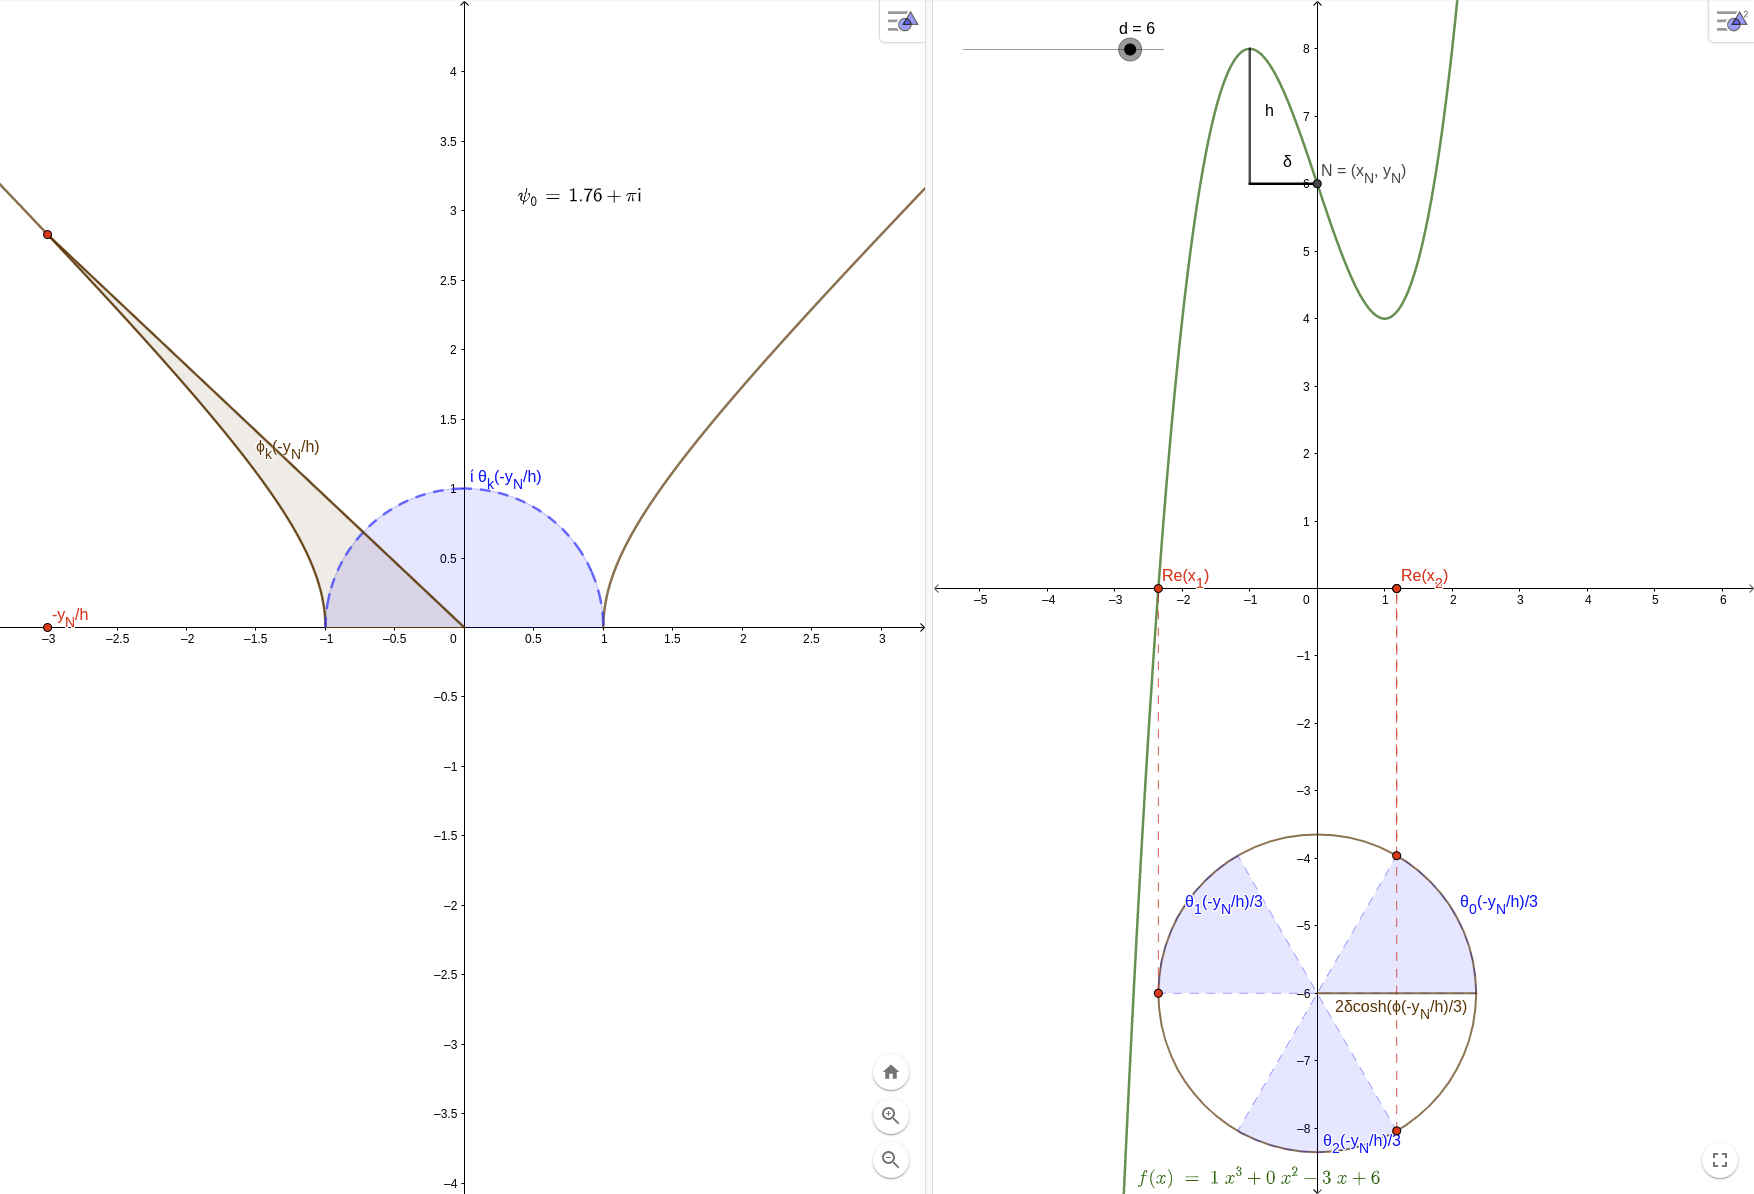
\includegraphics[width=\linewidth]{cubic_figure1.png}
	\caption{\mbox{$\psi_k\left(\dfrac{-y_N}{h}\right) \mathrm{ for } \dfrac{-y_N}{h} < -1$}, 1 real root, 2 complex roots} 
	\label{fig:angle1}
\end{figure}

\begin{figure}[h]
	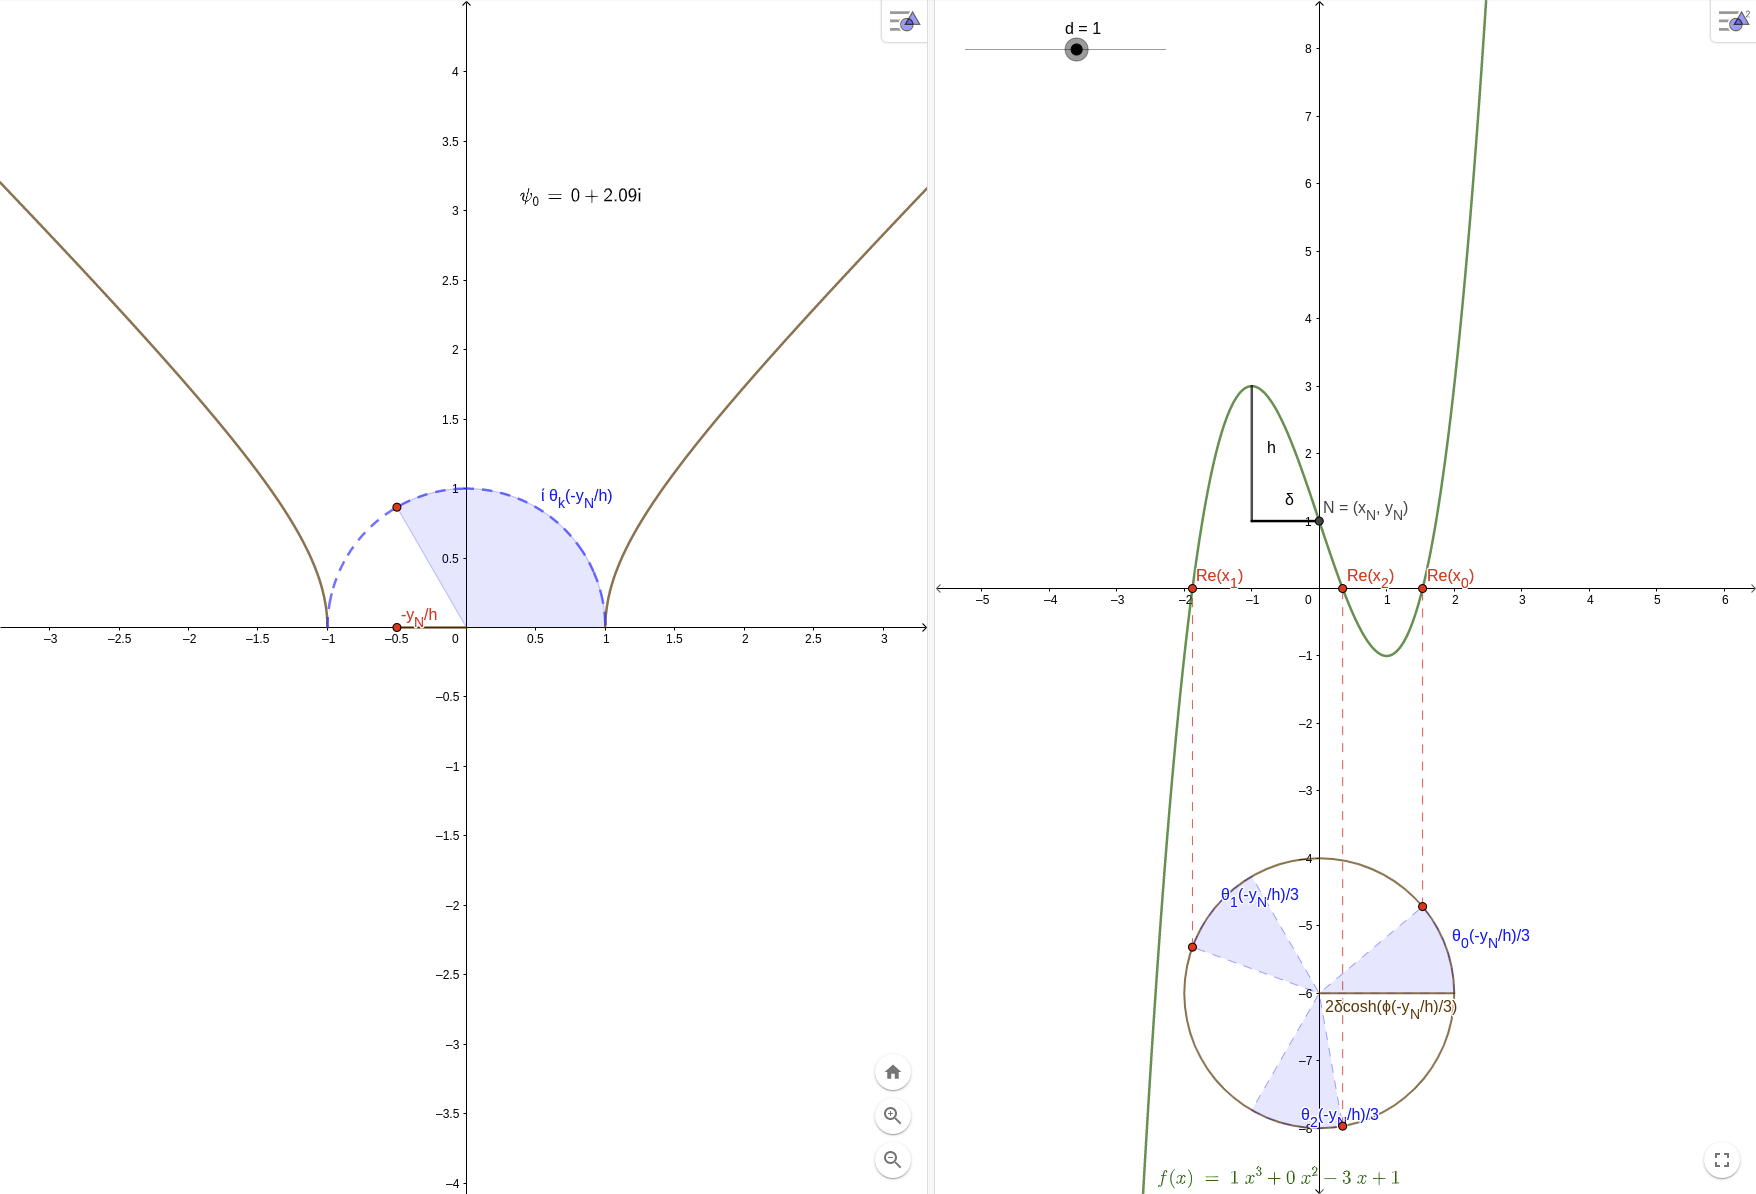
\includegraphics[width=\linewidth]{cubic_figure2.png}
	\caption{\mbox{$\psi_k\left(\dfrac{-y_N}{h}\right) \mathrm{ for } -1 \le \dfrac{-y_N}{h} \le 1$}, 3 real roots} 
	\label{fig:angle2}
\end{figure}

\clearpage
\section{Realtionship of the Hyperbolic Cosine Solutions to the Radical Solutions}
The following steps show how the expression for the roots of a cubic equation in terms of a complex hyperbolic angle relates to the expression for the roots in terms of radicals.

\begin{align*}
	x_k &= x_N + 2\delta\cosh\left[\dfrac{1}{3}\psi_k\left(\dfrac{-y_N}{h}\right)\right] \quad k \in \{0, 1, 2\} \\
	\\
	&= x_N + \delta e^{\frac{\psi_k\left(\frac{-y_N}{h}\right)}{3}} + \delta e^{\frac{-\psi_k\left(\frac{-y_N}{h}\right)}{3}} \quad k \in \{0,1,2\}\\
	\\
	&= x_N + \delta\sqrt[3]{e^{\psi_k\left(\frac{-y_N}{h}\right)}} + \delta\sqrt[3]{e^{-\psi_k\left(\frac{-y_N}{h}\right)}} \quad k \in \{0,1,2\}\\
	\\
	&= x_N + \delta\sqrt[3]{\cosh\left[\psi_k\left(\dfrac{-y_N}{h}\right)\right] + \sinh\left[\psi_k\left(\dfrac{-y_N}{h}\right)\right]} \\
	&\quad\quad\quad + \delta\sqrt[3]{\cosh\left[\psi_k\left(\dfrac{-y_N}{h}\right)\right] - \sinh\left[\psi_k\left(\dfrac{-y_N}{h}\right)\right]} \quad k \in \{0,1,2\}\\
	\\
	&= x_N + \delta\sqrt[3]{\cosh\left[\psi_k\left(\dfrac{-y_N}{h}\right)\right] + \sqrt{\cosh^2\left[\psi_k\left(\dfrac{-y_N}{h}\right)\right]-1}} \\
	&\quad \quad \quad + \delta\sqrt[3]{\cosh\left[\psi_k\left(\dfrac{-y_N}{h}\right)\right] - \sqrt{\cosh^2\left[\psi_k\left(\dfrac{-y_N}{h}\right)\right]-1}} \quad k \in \{0,1,2\}\\
	\\
	&= x_N + \delta\sqrt[3]{\dfrac{-y_N}{h} + \sqrt{\left(\dfrac{-y_N}{h}\right)^2-1}} + \delta\sqrt[3]{\dfrac{-y_N}{h} - \sqrt{\left(\dfrac{-y_N}{h}\right)^2-1}} \\
	\\
	&= x_N + \sqrt[3]{\dfrac{1}{2a}\left(-y_N + \sqrt{y_N^2 - h^2}\right)} + \sqrt[3]{\dfrac{1}{2a}\left(-y_N - \sqrt{y_N^2 - h^2}\right)}
\end{align*}

\newpage
\printbibliography

\end{document}
